% A LaTeX template for MSc Thesis submissions to 
% Politecnico di Milano (PoliMi) - School of Industrial and Information Engineering
%
% S. Bonetti, A. Gruttadauria, G. Mescolini, A. Zingaro
% e-mail: template-tesi-ingind@polimi.it
%
% Last Revision: October 2021
%
% Copyright 2021 Politecnico di Milano, Italy. NC-BY

\documentclass{Configuration_Files/PoliMi3i_thesis}

%------------------------------------------------------------------------------
%	REQUIRED PACKAGES AND  CONFIGURATIONS
%------------------------------------------------------------------------------

% CONFIGURATIONS
\usepackage{parskip} % For paragraph layout
\usepackage{setspace} % For using single or double spacing
\usepackage{emptypage} % To insert empty pages
\usepackage{multicol} % To write in multiple columns (executive summary)
\setlength\columnsep{15pt} % Column separation in executive summary
\setlength\parindent{0pt} % Indentation
\raggedbottom  

% PACKAGES FOR TITLES
\usepackage{titlesec}
% \titlespacing{\section}{left spacing}{before spacing}{after spacing}
\titlespacing{\section}{0pt}{3.3ex}{2ex}
\titlespacing{\subsection}{0pt}{3.3ex}{1.65ex}
\titlespacing{\subsubsection}{0pt}{3.3ex}{1ex}
\usepackage{color}

% PACKAGES FOR LANGUAGE AND FONT
\usepackage[english]{babel} % The document is in English  
\usepackage[utf8]{inputenc} % UTF8 encoding
\usepackage[T1]{fontenc} % Font encoding
\usepackage[11pt]{moresize} % Big fonts

% PACKAGES FOR IMAGES
\usepackage{graphicx}
\usepackage{transparent} % Enables transparent images
\usepackage{eso-pic} % For the background picture on the title page
\usepackage{subfig} % Numbered and caption subfigures using \subfloat.
\usepackage{tikz} % A package for high-quality hand-made figures.
\usetikzlibrary{}
\graphicspath{{./Images/}} % Directory of the images
\usepackage{caption} % Coloured captions
\usepackage{xcolor} % Coloured captions
\usepackage{amsthm,thmtools,xcolor} % Coloured "Theorem"
\usepackage{float}

% STANDARD MATH PACKAGES
\usepackage{amsmath}
\usepackage{amsthm}
\usepackage{amssymb}
\usepackage{amsfonts}
\usepackage{bm}
\usepackage[overload]{empheq} % For braced-style systems of equations.
\usepackage{fix-cm} % To override original LaTeX restrictions on sizes

% PACKAGES FOR TABLES
\usepackage{tabularx}
\usepackage{longtable} % Tables that can span several pages
\usepackage{colortbl}
\usepackage{multicol}

% PACKAGES FOR ALGORITHMS (PSEUDO-CODE)
\usepackage{algorithm}
\usepackage{algorithmic}

% PACKAGES FOR REFERENCES & BIBLIOGRAPHY
\usepackage[colorlinks=true,linkcolor=black,anchorcolor=black,citecolor=black,filecolor=black,menucolor=black,runcolor=black,urlcolor=black]{hyperref} % Adds clickable links at references
\usepackage{cleveref}
\usepackage[square, numbers, sort&compress]{natbib} % Square brackets, citing references with numbers, citations sorted by appearance in the text and compressed
\bibliographystyle{abbrvnat} % You may use a different style adapted to your field

% OTHER PACKAGES
\usepackage{pdfpages} % To include a pdf file
\usepackage{afterpage}
\usepackage{lipsum} % DUMMY PACKAGE
\usepackage{fancyhdr} % For the headers
\fancyhf{}
\usepackage{wrapfig}

% MY PACKAGES
\usepackage{changepage}
% Input of configuration file. Do not change config.tex file unless you really know what you are doing. 
% Define blue color typical of polimi
\definecolor{bluepoli}{cmyk}{0.4,0.1,0,0.4}

% Custom theorem environments
\declaretheoremstyle[
  headfont=\color{bluepoli}\normalfont\bfseries,
  bodyfont=\color{black}\normalfont\itshape,
]{colored}

% Set-up caption colors
\captionsetup[figure]{labelfont={color=bluepoli}} % Set colour of the captions
\captionsetup[table]{labelfont={color=bluepoli}} % Set colour of the captions
\captionsetup[algorithm]{labelfont={color=bluepoli}} % Set colour of the captions

\theoremstyle{colored}
\newtheorem{theorem}{Theorem}[chapter]
\newtheorem{proposition}{Proposition}[chapter]

% Enhances the features of the standard "table" and "tabular" environments.
\newcommand\T{\rule{0pt}{2.6ex}}
\newcommand\B{\rule[-1.2ex]{0pt}{0pt}}

% Pseudo-code algorithm descriptions.
\newcounter{algsubstate}
\renewcommand{\thealgsubstate}{\alph{algsubstate}}
\newenvironment{algsubstates}
  {\setcounter{algsubstate}{0}%
   \renewcommand{\STATE}{%
     \stepcounter{algsubstate}%
     \Statex {\small\thealgsubstate:}\space}}
  {}

% New font size
\newcommand\numfontsize{\@setfontsize\Huge{200}{60}}

% Title format: chapter
\titleformat{\chapter}[hang]{
\fontsize{50}{20}\selectfont\bfseries\filright}{\textcolor{bluepoli} \thechapter\hsp\hspace{2mm}\textcolor{bluepoli}{|   }\hsp}{0pt}{\huge\bfseries \textcolor{bluepoli}
}

% Title format: section
\titleformat{\section}
{\color{bluepoli}\normalfont\Large\bfseries}
{\color{bluepoli}\thesection.}{1em}{}

% Title format: subsection
\titleformat{\subsection}
{\color{bluepoli}\normalfont\large\bfseries}
{\color{bluepoli}\thesubsection.}{1em}{}

% Title format: subsubsection
\titleformat{\subsubsection}
{\color{bluepoli}\normalfont\large\bfseries}
{\color{bluepoli}\thesubsubsection.}{1em}{}

% Shortening for setting no horizontal-spacing
\newcommand{\hsp}{\hspace{0pt}}

\makeatletter
% Renewcommand: cleardoublepage including the background pic
\renewcommand*\cleardoublepage{%
  \clearpage\if@twoside\ifodd\c@page\else
  \null
  \AddToShipoutPicture*{\BackgroundPic}
  \thispagestyle{empty}%
  \newpage
  \if@twocolumn\hbox{}\newpage\fi\fi\fi}
\makeatother

%For correctly numbering algorithms
\numberwithin{algorithm}{chapter}

%----------------------------------------------------------------------------
%	NEW COMMANDS DEFINED
%----------------------------------------------------------------------------

\newcommand{\bea}{\begin{eqnarray}} % Shortcut for equation arrays
\newcommand{\eea}{\end{eqnarray}}
\newcommand{\e}[1]{\times 10^{#1}}  % Powers of 10 notation

%----------------------------------------------------------------------------
%	BEGIN OF YOUR DOCUMENT
%----------------------------------------------------------------------------

\begin{document}

\fancypagestyle{plain}{%
\fancyhf{} % Clear all header and footer fields
\fancyhead[RO,RE]{\thepage} %RO=right odd, RE=right even
\renewcommand{\headrulewidth}{0pt}
\renewcommand{\footrulewidth}{0pt}}

%----------------------------------------------------------------------------
%	TITLE PAGE
%----------------------------------------------------------------------------

\pagestyle{empty} % No page numbers
\frontmatter % Use roman page numbering style (i, ii, iii, iv...) for the preamble pages

\puttitle{
	title=eMall -- e-Mobility for all,
	nameA=Fabio Lusha - 10882532,
	nameB=Bianca C. Savoiu Marinas - 10684465,
	academicyear=2022-2023
}
\startpreamble
\setcounter{page}{1} % Set page counter to 1

%----------------------------------------------------------------------------
%	LIST OF CONTENTS/FIGURES/TABLES/SYMBOLS
%----------------------------------------------------------------------------

% TABLE OF CONTENTS
\thispagestyle{empty}
\tableofcontents % Table of contents 
\thispagestyle{empty}
\cleardoublepage

\addtocontents{toc}{\vspace{2em}} % Add a gap in the Contents, for aesthetics
\mainmatter % Begin numeric (1,2,3...) page numbering

% ----------------------
% CHAPTERS
% ----------------------

\chapter{Introduction}
\label{ch:chapter_one}%
\section{Purpose}
\label{sec:purpose}%
Widespread electrification of transport is the most efficient way to reach Europe’s climate objectives for the sector and electric charging is the main asset to overcome the obstacles of the take-up of electric vehicles (EVs). EVs can reduce CO2 by an estimated annual 600,000 tons by 2030, going towards a carbon neutral Europe, and the importance of this aim raises the problem of having efficient systems that manage the charging services. The eMall is thought as an all-encompassing application that oversees the entire process from the user interaction to the effective recharge of the EV's battery.

The main goal we want to achieve with the eMall software is to help The EVDs (electric vehicle drivers) to have a better access to recharge and to be able to book a charging point in order to avoid interference with his daily plans. Another important purpose of the system is to safeguard not only the users but also the providers of the service and this is made through privacy agreements and the actual interaction, that guarantees to supervise both interested parts, in order to get the best possible service and pay for it accordingly, having also a technical and economic exploitation of the charging infrastructures.

In this context there is an increase in the requested electric energy, but large amounts of power in short periods would require investments in the reinforcement of the distribution networks, which have not been designed to accommodate such load. It becomes necessary to introduce new systems and solutions to optimize the operation of the distribution networks. In this context we can identify the DSOs as the suppliers of electricity through the distribution networks. The DSOs interact with the eMall, and in particular with the CPMS (Charging Point Management System) module of the system to be. The CPMS, then, gives the information about the DSO's supply to the CPOs, which are important actors, that use the system in order to manage the charging service. A CPO is represented by an employee or a software, part of the business that owns some charging stations and wants to manage them through the eMall, deciding from where to acquire energy, and how to establish the prices, the special offers and other details about the stations.

The eMall is thought as a software that manages both the interaction with the businesses that offer the charging service and the interaction with the EVDs which want to use these services in order to charge their EVs. Therefore, the eMall provides a mobile application (eMma), which through its interface allows to the EVD to obtain the service, and provides, also, a web application that the CPOs use to manage the charging stations. The EVD interacts, as well, with the charging point interface (eMci), that communicates with the CPMS part of the eMall, in order to start the charging session from the station, plugging then the car to the compatible connector to effectively charge the EV.

\paragraph{Goals} In the following table we present the main goals of the software to be. The goals capture the needs of the stakeholders, which are the EVDs and the CPOs.

\newcounter{gc}
\setcounter{gc}{1}
\newcommand{\gcnt}{\thegc\stepcounter{gc}}
\begin{table}[H]
    \centering
    \begin{tabular}{|l|p{0.9\linewidth}|}
     \hline
     \textbf{Goal} & \textbf{Description} \\
     \hline
     G\gcnt & The EVD is able to identify the charging stations nearby \\
     \hline
     G\gcnt & The EVD is able to visualize the tariffs of the charging stations \\
     \hline
     G\gcnt & The EVD is able to visualize any special offer available at the charging station \\
     \hline
     G\gcnt & The EVD is able to book a charge in a specific charging station for a certain time frame\\
     \hline
     G\gcnt & The EVD is able to start the charging process at a certain station \\
     \hline
     G\gcnt & The EVD is able to pay for the obtained service \\
     \hline
     G\gcnt & The CPO can decide from which DSO to acquire energy \\
     \hline 
     G\gcnt & The CPO can decide the cost of charging \\
     \hline 
     G\gcnt & The CPO can set special offers \\
     \hline 
     G\gcnt & The CPO can decide whether to store or not energy in batteries \\
     \hline 
     G\gcnt & The CPO can decide whether to use the energy available in the batteries \\
     \hline 
\end{tabular}
    \caption{Goals}
    \label{tab:Goals}
\end{table}

\section{Scope}
\label{sec:Scope}%
\paragraph{World phenomena} The portion of the real world where the machine is to be deployed and used is called the environment. Hence, scoping the problem by defining the environment is paramount, and this is the target of the next table. With the world phenomena we define the environment in which the software to be will operate, by clarifying some facts about the world and the users. In the following chapter, to the environment will be also given some boundaries, making some assumptions and describing some domains properties, but this is not an aspect tackled by the next table of phenomena.
\newcounter{wp}
\setcounter{wp}{1}
\newcommand{\wpcount}{\thewp\stepcounter{wp}}
\begin{center}
    \begin{longtable}{|l|p{0.725\linewidth}|}
     \hline
     \textbf{World phenomena} & \textbf{Description} \\
     \hline
     WP\wpcount & The EVD wants to charge the EV's battery \\
     \hline
     WP\wpcount & The EVD wants to plan where and when to charge the EV's battery, so he needs to know the position on the territory of the charging stations and if there are available and compatible charging points\\
     \hline
     WP\wpcount & The EVD wants to know the price and any special offers of the charging stations, to choose the one that better suits his needs \\
     \hline
     WP\wpcount & The prices of energy often vary in real world economy \\ 
     \hline
     WP\wpcount & The DSOs, as marketing strategy, have special offers during certain time periods.\\
     \hline
     WP\wpcount & The DSOs provide energy to the charging stations \\
     \hline
     WP\wpcount & The DSOs decide the energy price\\
     \hline
     WP\wpcount & The providers of the charging service (CPOs) make special offers during certain time periods\\
     \hline
     WP\wpcount & The CPOs decide the price of charging, following marketing trends, and depending on DSOs prices and business decisions\\
     \hline
     WP\wpcount & EVs may have an integrated rectifier that converts AC electricity to DC \\
     \hline
     WP\wpcount & Some type of chargers have an integrated rectifier that converts AC electricity to DC. They supply the EV directly with DC current \\
     \hline
     WP\wpcount & A charging of type X, provides electricity in mode C and is given through Z connectors \\
     \hline
     WP\wpcount & A charging station is owned and managed by one CPO \\
     \hline
     WP\wpcount & A CPO owns and manages one or more charging stations \\
     \hline
     WP\wpcount & The CPO buys energy from the DSOs\\
     \hline
     WP\wpcount & A charging station may be equipped with batteries \\
     \hline
     WP\wpcount & Charging stations equipped with batteries grant more flexibility to CPOs on how to choose between the energy stored in the batteries and the one offered by DSOs \\
     \hline
     WP\wpcount & Low voltage (3.7 - 11 kW) chargers need more time to charge the battery \\
     \hline
     WP\wpcount & Medium voltage (22-90 kW) chargers need less time to recharge a battery of capacity C than a low voltage charger \\
     \hline
     WP\wpcount & High voltage (> 90 kW) chargers need less time to recharge a battery of capacity C than a medium voltage charger \\
     \hline
     WP\wpcount & Batteries can only be charged with direct current (DC) electric power \\
     \hline
     WP\wpcount & Given a continuous supply of power W, and a battery with finite capacity C, than the charging time T is finite. \\
     \hline
     WP\wpcount & A battery can store a finite amount of energy, given by its capacity C. \\
     \hline
     WP\wpcount & The charging point of a specific charging station may be unusable because of maintenance or faults \\
     \hline
     WP\wpcount & The DSOs distribute and manage energy from the generation sources\\
     \hline
     WP\wpcount & Most electricity is delivered from the power grid as alternating current (AC) \\
     \hline
     WP\wpcount & During the day the electric power supplied to the station can vary\\
     \hline
     WP\wpcount & During the day a short-duration reduction in the voltage supplied to the electrical power systems may occur due to high current demand or faults in the system.\\
     \hline
     WP\wpcount & During the day a momentary increase in voltage may occur. This may happen when a heavy load turns off in a power system.\\
     \hline
     WP\wpcount & The DSOs operate and manage the electricity distribution networks\\ 
     \hline
     WP\wpcount & The DSOs solve grid problems, such as faults and network breaks\\
     \hline
    \caption{World Phenomena}
    \label{tab:World Phenomena}
    \end{longtable}
\end{center}

\paragraph{Shared phenomena} The shared phenomena define the interface through which the machine interacts with the world. The software monitors some shared phenomena, while controls others, and to show when the software takes the part of the controller and when the part of the observer we created two more columns in the next table, to keep track of the initiator of the action, in case the natural language turns out to be ambiguous. So, in the following assertions we present an interaction between the world (users and external systems) and the machine (the eMall, especially its interfaces, such as the eMma, the eMci and the managerial web application).  
%TODO: In the SP substitute the eMall with the specific interfaces that takes part in the shared phenomena

\newcounter{sp}
\setcounter{sp}{1}
\newcommand{\spcount}{\thesp\stepcounter{sp}}
\begin{center}
    %\centering
    \begin{longtable}[H]{|p{0.15\linewidth}|p{0.41\linewidth}|p{0.15\linewidth}|l|}
     \hline
     \textbf{Shared phenomena} & \textbf{Description} & \textbf{Controller} & \textbf{Observer} \\
     \hline
     SP\spcount & The eMall notifies the EVD when the charging process is finished & eMall & EVD\\
     \hline
     SP\spcount & The EVD creates an account & EVD & eMall\\
     \hline
     SP\spcount & The EVD in order to register inserts in the mobile app of the eMall the personal data (name, surname, email, password, payment details) & EVD & eMall \\
     \hline
     SP\spcount & The EVD logs in using the email and the password & EVD & eMall\\
     \hline
     SP\spcount & The EVD accepts the terms of service in order to use the eMma & EVD & eMall\\
     \hline
     SP\spcount & The EVD shares its location with the eMall & EVD & eMall\\
     \hline
     SP\spcount & The EVD confirms the payment from the mobile application of the eMall & EVD & eMall \\
     \hline
     SP\spcount & The EVD deletes previously inserted EVs from its account & EVD & eMall\\
     \hline
     SP\spcount & The EVD updates the specifications of the EVs on its account & EVD & eMall \\
     \hline
     SP\spcount & The EVD adds a new EV to its account & EVD & eMall \\
     \hline
     SP\spcount & The EVD inserts the maximum and minimum current supported by the EV & EVD & eMall \\
     \hline
     SP\spcount & The EVD inserts the maximum power supported by the EV & EVD & eMall \\
     \hline
     SP\spcount & The EVD inserts the inlet type of the EV & EVD & eMall \\
     \hline
     SP\spcount & The EVD inserts whether the EV is equipped with a built-in rectifier & EVD & eMall \\
     \hline
     SP\spcount & The EVD inserts the capacity of the battery in kWh & EVD & eMall \\
     \hline
     SP\spcount & The eMall shows to the EVD the map of the charging stations nearby his location & eMall & EVD \\
     \hline
     SP\spcount & The EVD chooses a charging station from the map & EVD & eMall \\
     \hline
     SP\spcount & The eMall shows the user the rating of the charging station & eMall & EVD \\
     \hline
     SP\spcount & The EVD inserts the expected time when he plans to start the charging process & EVD & eMall \\
     \hline
     SP\spcount & The EVD inserts the expected time when he plans to end the charging process & EVD & eMall \\
     \hline
     SP\spcount & The eMall shows to the EVD the list of available chargers of the charging station & eMall & EVD \\
     \hline
     SP\spcount & The eMall shows the charger type and its connectors  & eMci / eMma & EVD  \\
     \hline
     SP\spcount & The EVD chooses the charger he wants to use from the list of available ones & EVD & eMall \\
     \hline
     SP\spcount & The eMall shows to the EVD the charger costs (per kWh, per minute, additional costs) & eMma/eMci & EVD \\
     \hline
     SP\spcount & The eMall shows to the EVD the status of the charger & eMci & EVD \\
     \hline
     SP\spcount & The eMall shows to the EVD the battery level of the connected EV & eMci & EVD \\
     \hline
     SP\spcount & During the charging session the eMall shows to the EVD the power output of the charger & eMci & EVD \\
     \hline
     SP\spcount & During the charging session the eMall shows to the EVD the remaining time to complete the charging process & eMci & EVD \\
     \hline
     SP\spcount & The EVD starts the charging session from the charger & EVD & eMSP\\
     \hline
     SP\spcount & \textit{The CPMS asks the DSO about the current available energy sources, their prices, and special offers} & CPMS & DSO \\ %Requirement
     \hline
     SP\spcount & The DSO dynamically changes the price of electricity & DSO & CPMS \\
     \hline
     SP\spcount & The DSO changes dynamically the \textit{energy sources} from which acquires energy & DSO & CPMS \\
     \hline
     SP\spcount & The DSO makes special offers & DSO & CPMS \\
     \hline
     SP\spcount & The CPO logs in & CPO & CPMS \\
     \hline
     SP\spcount & The CPO selects the charging station for which to set the parameters (price, energy) of the charging service & CPO & CPMS \\
     \hline
     SP\spcount & The CPO selects the DSO from which to acquire energy & CPO & CPMS \\
     \hline
     SP\spcount & The CPMS shows to the CPO the \textit{energy sources} and the relative current prices and special offers of the DSO & CPMS & DSO \\
     \hline
     SP\spcount & The CPO sets the cost of charging & CPO & CPMS \\
     \hline
      SP\spcount & The CPO can set a special offer & CPO & CPMS \\
     \hline
     SP\spcount & The CPO selects the energy sources from which to acquire energy & CPO & CPMS \\
     \hline
     SP\spcount & The CPMS shows if there are available batteries in the charging station & CPMS & CPO \\
     \hline
     SP\spcount & The CPO selects the battery in which to store energy & CPO & CPMS \\
     \hline
     SP\spcount & The CPO sets the amount of energy to store in the battery & CPO & CPMS \\
     \hline
     SP\spcount & The CPMS dynamically shows to the CPO the number of EVs charging & CPMS & CPO \\
     \hline
     SP\spcount & The CPMS dynamically shows to the CPO the charging stations consumption of energy & CPMS & CPO \\
     \hline
    \caption{Shared Phenomena}
    \label{tab:Shared Phenomena}
    \end{longtable}
\end{center}
% TODO: Add SP for the EVSE events (it breaks during charging, an error occurs etc)

\section{Definitions, Acronyms, Abbreviations}
\label{sec:Definitions, Acronyms, Abbreviations}%
\subsection{Abbreviations}
\begin{itemize}
    \item \textbf{eMall}: e-Mobility for all
    \item \textbf{eMma}: e-Mall mobile application
    \item \textbf{eMci}: e-Mall charger interface
    \item \textbf{CPMS}: Charging Point Management System
    \item \textbf{CPO}: Charge Point Operator
    \item \textbf{eMSP}: Electric Mobility Service Providers
    \item \textbf{DMS}: Distribution Management System
    \item \textbf{DSO}: Distribution System Operator
    \item \textbf{EV}: Electric Vehicle
    \item \textbf{EVD}: Electric Vehicle Driver
    \item \textbf{EVSE}: Electric Vehicle Supply Equipment
    \item \textbf{HV}: High Voltage
    \item \textbf{LV}: Low Voltage
    \item \textbf{MV}: Medium Voltage
    \item \textbf{SCADA}: Supervisory Control and Data Acquisition
    \item \textbf{SCM}: Smart Charging Management 
    \item \textbf{OMS}: Outage Management System
    \item \textbf{AC}: Alternating current
    \item \textbf{DC}: Direct current
\end{itemize}

\subsection{Definitions}
\begin{itemize}
    \item \textbf{DSO}: typically the entity responsible for the operation and management of distribution networks – High, Medium and Low Voltage networks. For this purpose, the DSO typically owns systems such as Supervisory and Control Data Acquisition (SCADA)/ Distribution Management System (DMS) for the monitoring and general overview of the state of the network. It also owns other systems such as the Outage Management System (OMS) and Work Force Management System (WFMS) for addressing the network operation problems related with the continuity and quality of service.
    \item \textbf{CPO}: entity that technically manages all the EV infrastructure assets, depending of existing country regulation – this role can be assured by the DSO or other entity.
    \item \textbf{eMSP}: is the entity that can explore the economic side of the EV charging infrastructure, namely by selling energy for charging purposes.
    \item \textbf{CPMS}: is a software system that manages the charge point infrastructure – can manage the technical and economic aspects of the charging infrastructures.
    \item  \textbf{EVD}: person or entity who owns an EV car and can use the public or private facilities for charging purposes.
    \item \textbf{EVSE}: Electric Vehicle Supply Equipment. It is an equipment that is able to charge EV batteries with AC or DC loads and with different rated powers depending on the type of equipment.
    % TODO: what does this mean (private parking)
    \item  \textbf{Private parking}: can be a condominium, industry or other entity who has private owned EV
    \item \textbf{Voltage sag}: a short-duration reduction in voltage of an electric power distribution system. It can be caused by high current demand or fault current elsewhere in the system.
    \item \textbf{Voltage swell}: the opposite of voltage sag. Voltage swell, which is a momentary increase in voltage, happens when a heavy load turns off in a power system.
    \item \textbf{Socket outlet}: the port on the electric vehicle supply equipment (EVSE) that supplies charging power to the vehicle
    \item \textbf{Plug}: the end of the flexible cable that interfaces with the socket outlet on the EVSE.
    \item \textbf{Cable}: a flexible bundle of conductors that connects the EVSE with the electric vehicle
    \item \textbf{Connector}: the end of the flexible cable that interfaces with the vehicle inlet
    \item \textbf{Vehicle inlet}: the port on the electric vehicle that receives charging power
    \item \textit{Inverter}: It is a power electronic device or circuitry that changes direct current (DC) to alternating current (AC).
    \item \textbf{Rectifier}: an electrical device that converts alternating current (AC) to direct current (DC).
    \item \textbf{eMma}: the eMSP subsystem responsible for the EVD interaction from the mobile app
    \item \textbf{eMci}: the eMSP subsystem responsible for the EVD interaction at the charging point
    \textit{ \item \textbf{additional costs}: overtime penalty, deposit for unregistered users}
    \item \textbf{Status of the charger}: can be free, occupied, booked and in maintenance
    \item \textbf{Smart meter}: is an electronic device that records information such as consumption of electric energy, voltage levels, current, and power factor; allow the reading of energy flow and real-time usage, and consequently permit the identification of interruptions in energy flow
\end{itemize}

\section{Reference Documents}
\label{sec:Reference Documents}%
\begin{itemize}
    \item \verb|IEEE 29148-2018 International Standard - Requirements engineering|: defines the construct of a good requirement and provides attributes and characteristics of requirements; provides also additional guidelines for applying the requirements and requirements-related processes
    \item \verb|RDD| assignment document
    \item \verb|Electric Vehicle CPMS and Secondary Substation Management by F. Campos,| \verb|Efacec, Portugal; L. Marques, Efacec, Portugal and K. Kotsalos,| \verb|Efacec,| \verb|Portugal (15 October 2018)|: used to define the interactions between the different parts of the system and the actors; models the EV public infrastructures, the eMSP, the DSO and the CPMS together with the APIs and protocols that allow their communication
    \item \verb|EV CHARGING: HOW TO TAP IN THE GRID SMARTLY? by Platform |\verb|for|\\\verb|Electromobility| \verb|(May 2022)|: used to understand the environment of the problem and contextualize the analysis
\end{itemize}

\section{Document Structure}
\label{sec:Document Structure}%
This document mainly follows the guidelines of the \verb|IEEE 29148-2018 - International| \verb|Standard - Requirements engineering|, with some changes in the order of the contents. Also in the final part of the document is present an \verb|Alloy| formal analysis of the described model, an additional section with respect to the standard.
The document is composed by the following parts:
\begin{itemize}
    \item An introduction to the domain in which the system will operate (world phenomena) and an initial description of the software to be, the eMall, specifying the goals to achieve
    \item The overall description of the functions that the eMall has to implement specifying the requirements and a domain model, its interaction with the different users describing with diagrams the most important shared phenomena, and the domain assumptions necessary to the system to be
    \item A thorough list of requirements both functional and non functional: giving a detailed description of the functional requirements using use cases, use cases diagrams and UML sequence diagrams to better specify the interactions; and characterizing the non functional requirements through software system attributes
    \item A formal analysis using alloy in order to show the soundness and correctness of the model described in the document, considering only a part the most important requirements of the system
    \item A section that contains the effort spent by the members of the group working towards the completion of this document
\end{itemize}


\chapter{Overall description}
\label{ch:chapter_two}%
\section{Product perspective}
\label{sec:product_perspective}%

\section{Product functions}
\label{sec:Product functions}%

\section{User characteristics}
\label{sec:User_characteristics}%

\section{Assumptions, dependencies and constraints}
\label{sec:Assumptions, dependencies and constraints}%
\newcounter{ac}
\setcounter{ac}{1}
\newcommand{\acount}{\theac\stepcounter{ac}}
\begin{table}[h!]
    \centering
    \begin{tabular}{|l|p{0.725\linewidth}|}
     \hline
     \textbf{Assumptions} & \textbf{Description} \\
     \hline
     A\acount & The end user has internet connection \\
     \hline
     A\acount & The end user has a mobile phone with an integrated GPS module \\
     \hline
     A\acount & The end user has the mobile application of the eMSP installed on his mobile phone \\
     \hline
     A\acount & The CPMS shares the location of the charging station to the eMSP through APIs\\
     \hline
     A\acount & The end user payment from the mobile app is handled by external APIs.\\
     \hline
     A\acount & The EVD that creates an account inserts the personal data and the EVs specifications during registration \\
     \hline
     A\acount & The non registered EVD inserts the EVs specifications and payment details during the booking phase \\
     \hline
\end{tabular}
    \caption{Assumptions}
    \label{tab:Assumptions}
\end{table}

\chapter{Specific requirements}
\label{ch:chapter_three}%
\section{External Interface Requirements}
\label{sec:External Interface Requirements}%

\subsection{User Interfaces}
\label{sec:user interfaces}%
In this subsection we provide some mockups that show an example of some possible user interface, one for the mobile app which will be available to the users and one for the web app available to the businesses, that offer the charging service.

\paragraph{EVD interaction with the mobile app of the eMall}
The EVD needs to download the mobile app on his cellphone in order to interact with the eMall and take advantage of its functionalities. The Graphical User Interface (GUI) of the application is thought as an user-friendly interface, to facilitate everyone in using the service. In this first mockup we see the initial page of the system, shown to the user when opening the application.
\begin{figure}[H]
    \centering
    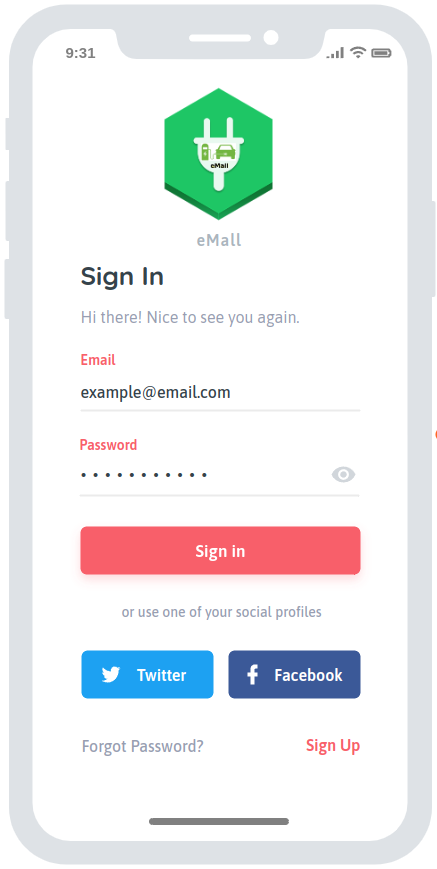
\includegraphics[scale=.3]{Images/cp3/signIn.png}
    \caption{Wireframe of the page that allows to log in from the eMma}
\end{figure}

In the following mockups we represent an example of the signing up procedure, showing the data required by the eMma in order to complete the creation of an account. 
\begin{figure}[H]
    \centering
    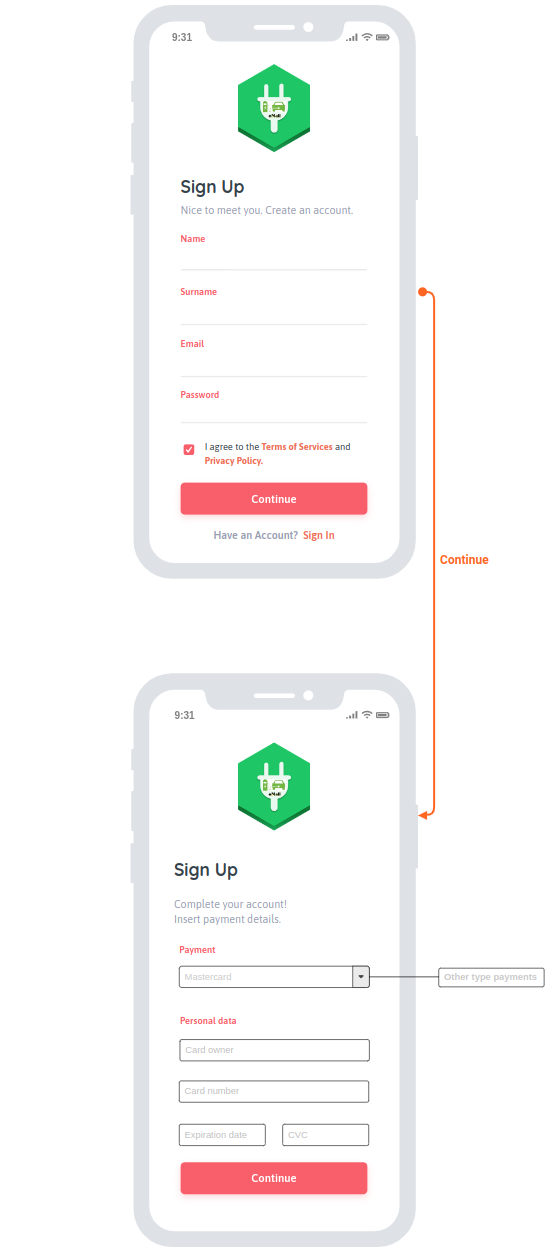
\includegraphics[scale=.45]{Images/cp3/signUp.png}
    \caption{Wireframe of the signing up process that allows to register from the eMma}
\end{figure}

\paragraph{CPO interaction with the managerial web app of the eMall}



\subsection{Hardware Interfaces}
\subsection{Software Interfaces}
\subsection{Communication Interfaces}

\section{Functional Requirements}
\label{sec:Functional Requirements}%

\section{Performance Requirements}
\label{sec:Performance Requirements}%

\section{Design Constraints}
\label{sec:Design Constraints}%

\subsection{Standards compliance}
\subsection{Hardware limitations}
\subsection{Any other constraint}

\section{Software System Attributes}
\label{sec:Software System Attributes}%

\subsection{Reliability}
\subsection{Availability}
\subsection{Security}
\subsection{Maintainability}
\subsection{Portability}


\chapter{Formal analysis using Alloy}
\label{ch:chapter_four}%
In this final section we present a formal specification of some of the requirements explained before. Using the Alloy analyzer we provide a description of the model and we try to prove its correctness and consistency. In particular, we show some constraints of the world in which the system to be will operate, and some functionalities. The objective driving this modeling phase was to verify that the model we have in mind regarding bookings and charging sessions respect the main overlapping constraints of the world. At the end of this section we also provide some visualizations of the obtained result, further explaining the satisfied requirements.

\begin{lstlisting}[frame = single]
open util/ordering[DateTime]

sig DateTime{}

// some actors in the system
abstract sig User {}

//We don't consider dangling elements 
sig Email{}{
	this in EVD.email
}
sig Password{}{
	this in EVD.password
}
sig Location{}{
	this in ChargingStation.location
}
sig History{
}{
	this in EVD.chargingHistory
}

sig EVD {
	evs: some EV,
    email: one Email, 
	password: one Password,
	chargingHistory: one History
}

sig DSO {}{
	this in ChargingStation.dso
}

abstract sig Socket {}
one sig Type1, Type2, Chademo extends Socket{}

sig EV {
	socket: one Socket,
}{
	this in EVD.evs
}

sig ChargingPoint {
 	socket: some Socket,
	connectedEV: lone EV
}{
	EV.socket in socket
	this in ChargingStation.chargingPoints
}

sig ChargingStation {
	chargingPoints: some ChargingPoint,
	location: one Location,
	dso: one DSO
}{
	this in CPO.chargingStations
}

sig CPO extends User{
	chargingStations: some ChargingStation
}

sig Booking {
	ev: EV,
	cs: ChargingStation,
	cp: ChargingPoint,
	start: DateTime,
	end: DateTime
}{
	// Only Registerd User can book
	ev in EVD.evs &&
	cp in cs.chargingPoints
	lt[start, end]
}

/*********** FACTS  *************/
//A charging point can belong only to a charging station
fact eachChargingToOnlyOneChargingStation{
	all disj x, y : ChargingStation |
		 #(x.chargingPoints & y.chargingPoints) = 0
}

//A charging station can be managed only by a CPO
fact eachCStoOnlyOneCPO{
	all disj x, y : CPO |
		 #(x.chargingStations & y.chargingStations) = 0
}

//An EV can belong to only an EVD
fact eachEVtoOnlyOneEVD {
	all disj x, y : EVD |
		 #(x.evs & y.evs) = 0
}

//The EV in a certain moment can be connected to only a charging point to charge
fact eachEVConnectedToOneChargingPoint{
    all disj x, y: ChargingPoint |
		 #(x.connectedEV & y.connectedEV) = 0
}

//Impose that there must not exist multiple bookings for the same vehicles at the same time
fact noEVOverBooking{
	no disj b1, b2: Booking
	| b1.ev = b2.ev && 
 		(gte[b1.start, b2.start] && lte[b1.start, b2.end] ||
 		 gte[b1.end, b2.start] && lte[b1.end, b2.end])
}

//Impose that there must not exist multiple bookings for the same charging point at the same time
fact noOverBooking{
	no disj b1, b2: Booking
	| b1.cp = b2.cp && 
		(gte[b1.start, b2.start] && lte[b1.start, b2.end] ||
		 gte[b1.end, b2.start] && lte[b1.end, b2.end])
}

//Only an EV can be in charge for an EVD in a certain moment
fact onlyAnEVisChargingForEVD{
	all evd: EVD, disj ev1, ev2 :EV |
	ev1 in evd.evs and ev2 in evd.evs and ev1 in ChargingPoint.connectedEV
	implies ev2 not in ChargingPoint.connectedEV
}

//Unique email to EVD
fact uniqueEmail{
 no disj driver1, driver2: EVD |
 	 driver1.email = driver2.email 
}

//Unique history to EVD
fact uniqueHistory{
 no disj driver1, driver2: EVD |
 	 driver1.chargingHistory = driver2.chargingHistory
}

//Unique location to ChargingStation
fact uniqueLocation{
 no disj cs1, cs2: ChargingStation |
 	 cs1.location = cs2.location
}

/**** ASSERTIONS ****/
//The same charging point can't be in two different charging stations
assert noCPinTwoChargingStations{
	no cp: ChargingPoint, disj cs1, cs2: ChargingStation | 
		cp in cs1.chargingPoints && cp in cs2.chargingPoints
}

//The same charging station can't be managed by two different CPOs
assert NoCSInTwoCPO{
 no cs: ChargingStation, disj CPO1, CPO2: CPO |
	cs in CPO1.chargingStations && cs in CPO2.chargingStations
}

//There is no charging point that doesn't belong to a charging station, because it's an entity that doesn't exist on its own in our system
assert notExistsCPnotInCS{
	no cp: ChargingPoint
	| cp not in ChargingStation.chargingPoints
}

//There is no EV that doesn't belong to a EVD, because it's an entity that doesn't exist on its own in our system
assert existsEVnotInRegEVD{
	some ev: EV
	| ev not in EVD.evs
}

//The booking has to regard an EV that belongs to the EVD, so an unregistered EVD cannot use this functionality, because the system is not able to keep track of its vehicles, and furthermore we also check that a booking cannot regard an EV that doesn't exist in the list of vehicles of the EVD
assert noBookingForUnregEVD{
	Booking.ev in EVD.evs
}

//There are no overlapping bookings for the same vehicle
assert noEVOverBooking{
	no disj b1, b2: Booking |
	b1.ev = b2.ev && gte[b1.start, b2.start] && lte[b1.start, b2.end]
}

//There are no overlapping bookings for the same charging point in the system, to maintain consistency and assure a correct service
assert bookingStartLessThanBookingEnd{
	all b: Booking | lt[b.start, b.end]
}

//Using the check we can see if Alloy finds some counterexamples of an assertion, checking the consistency of the world
check noCPinTwoChargingStations

/*********PREDICATES*********/
pred findBookings{
	some disj b1, b2: Booking | lt[b2.end, b1.start]
}

//Is possible to add an EV to the EVD
pred addEVToEVD[evd', evd: EVD, NewEv: EV]{
	evd'.evs = evd.evs + NewEv
}

//Is possible to add a charging station to the ones managed by a CPO
pred addCSToCPO[cpo', cpo: CPO, NewCS: ChargingStation]{
    cpo'.chargingStations = cpo.chargingStations + NewCS
}

//Is possible to delete a charging station from the ones managed by a CPO
pred deleteCSFromCPO[cpo', cpo: CPO, cs: ChargingStation]{
    cpo'.chargingStations = cpo.chargingStations - cs
}

//Is possible to add a charging point to a charging station, related to the CPO that manages it
pred addCPToCS[cs', cs:ChargingStation, cp: ChargingPoint, cpo, cpo': CPO]{
	cs in cpo.chargingStations
    cs'.chargingPoints = cs.chargingPoints + cp
	cpo'.chargingStations = cpo.chargingStations + cs'
}

//We show the task that the CPO wants to perform on the charging station, adding a new charging point, showing the case in which we already have other charging points, so we are not initializing the charging station, we are just updating it with new information
pred showAddCPToCS [cs', cs:ChargingStation, cp: ChargingPoint, cpo, cpo': CPO]{
	addCPToCS[cs', cs, cp, cpo, cpo']
	#(cs'.chargingPoints) > 2
}

//Dynamic model
run showAddCPToCS for 20 but exactly 3 ChargingStation

//To show the CPO interaction with the system
pred CPOworld{
	#CPO >= 2
	#ChargingStation >= 2
	#ChargingPoint >= 5
}

run CPOworld for 20

//To show the RegEVD interaction with the system
pred EVDworld{
	#EVD >= 2
	#EV >= 3
	#ChargingPoint >= 2
	#ChargingStation >= 1
	#Booking >= 1
}

run EVDworld for 10

run {} 
\end{lstlisting}

%TODO: a little explanation for each world important elements
\subsection{Resulting worlds}
\paragraph{The world mainly from the CPO point of view}
From the CPO point of view we show the following world generated with the Alloy analyzer, noticing some important requirements of the eMall:
\begin{itemize}
    \item The CPO manages one or more charging stations
    \item The charging stations have one ore more charging points
    \item The charging points can have different socket types (in the following representation Alloy generated a case in which each charging point has only a socket of one type, but in general the charging point can have many sockets of different types, but we assume that only one is used at the time)
    %TODO: add assumption only a socket is used at the time
    \item The charging stations acquire energy from different DSOs chosen by the CPO, and different charging stations, even of different CPOs, can acquire energy from the same DSO 
\end{itemize}
We can see a simple representation of these elements in the CPOworld:
\begin{figure}[H]
    \centering
    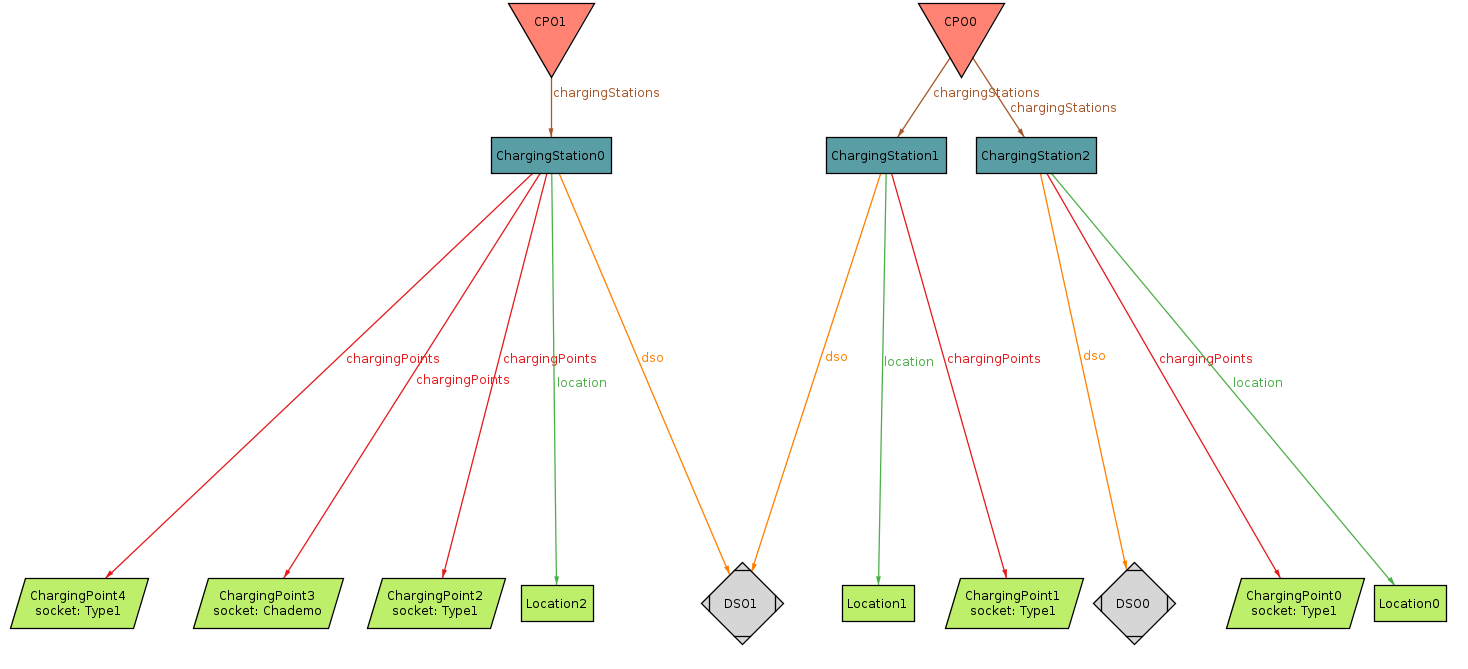
\includegraphics[width=1\textwidth]{Images/cp4/CPOWorld.png}
    \caption{A representation of the world from the CPO point of view}
\end{figure}

%TODO: in the Alloy connect the history with the chargings and the bookings
\paragraph{The world mainly from the EVD point of view}
To represent the EVD point of view we show a couple of worlds generated by the Alloy analyzer, in order to verify some requirements: 
\begin{itemize}
    \item The EVD has a mail and a password that he uses to log in
    \item The EVD has a charging history of his activities
    \item The EVD has one or more EVs, at least one because we assume that during registration phase the driver inserts a vehicle
    \item The EVD can have one or more bookings regarding an EV, but without overlapping time-frames
    \item There can be more bookings for a charging point, but without overlap in the time-frame chosen for the charging session
    \item An EVD can use the charging points, even without a booking
\end{itemize}

In the following two representations we can notice that the elements just explained are present and satisfied.
\begin{figure}[H]
    \centering
    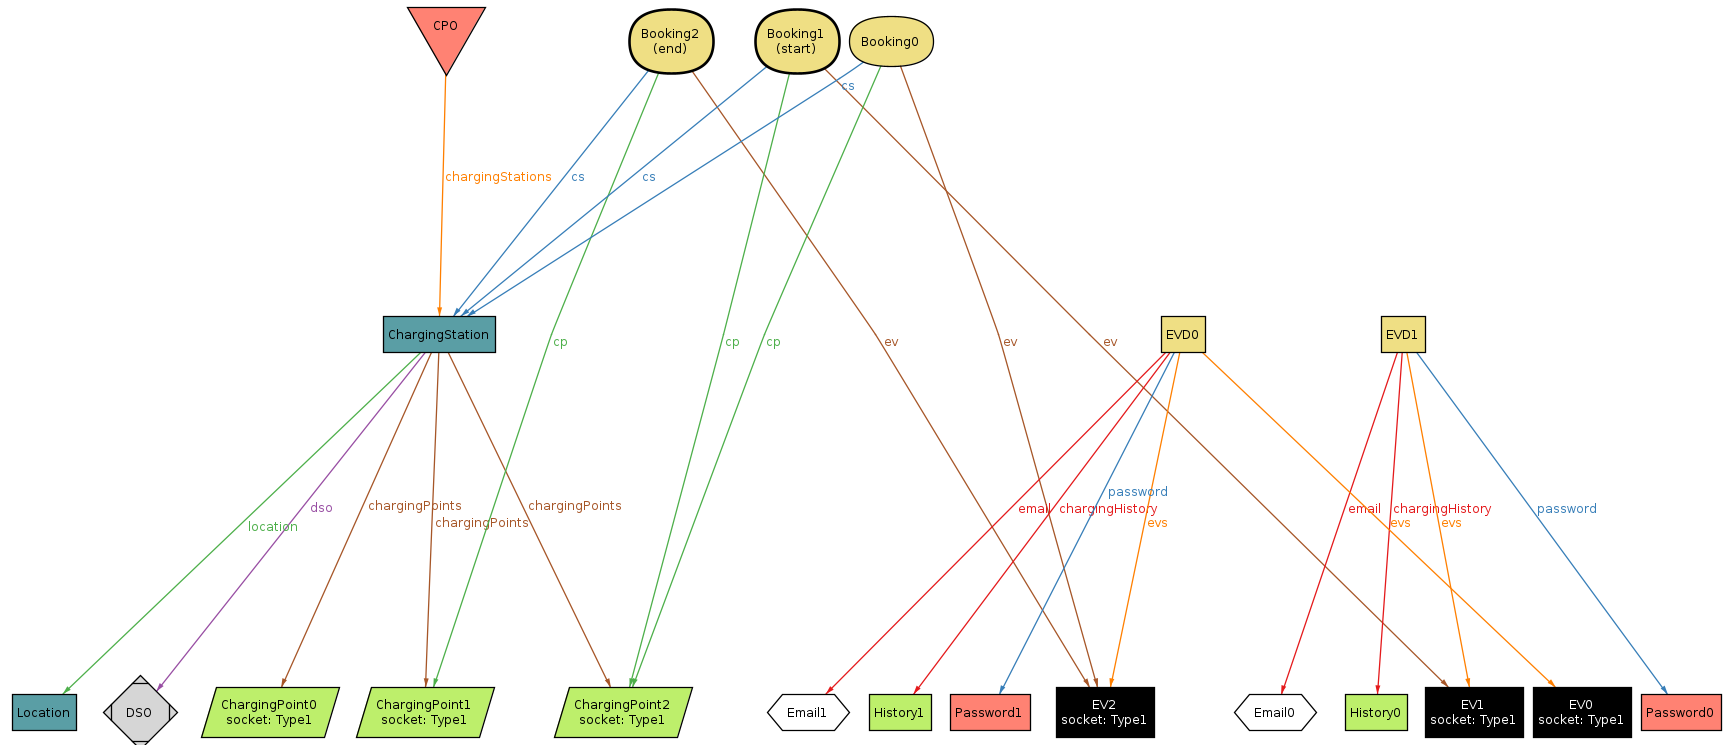
\includegraphics[width=1\textwidth]{Images/cp4/EVDWorldBooking.png}
    \caption{A first representation of the world from the EVD point of view}
\end{figure}

%TODO: in the Alloy add a time in using the charging point in the charge now case (free/occupied and in maintance CP?)
\begin{figure}[H]
    \centering
    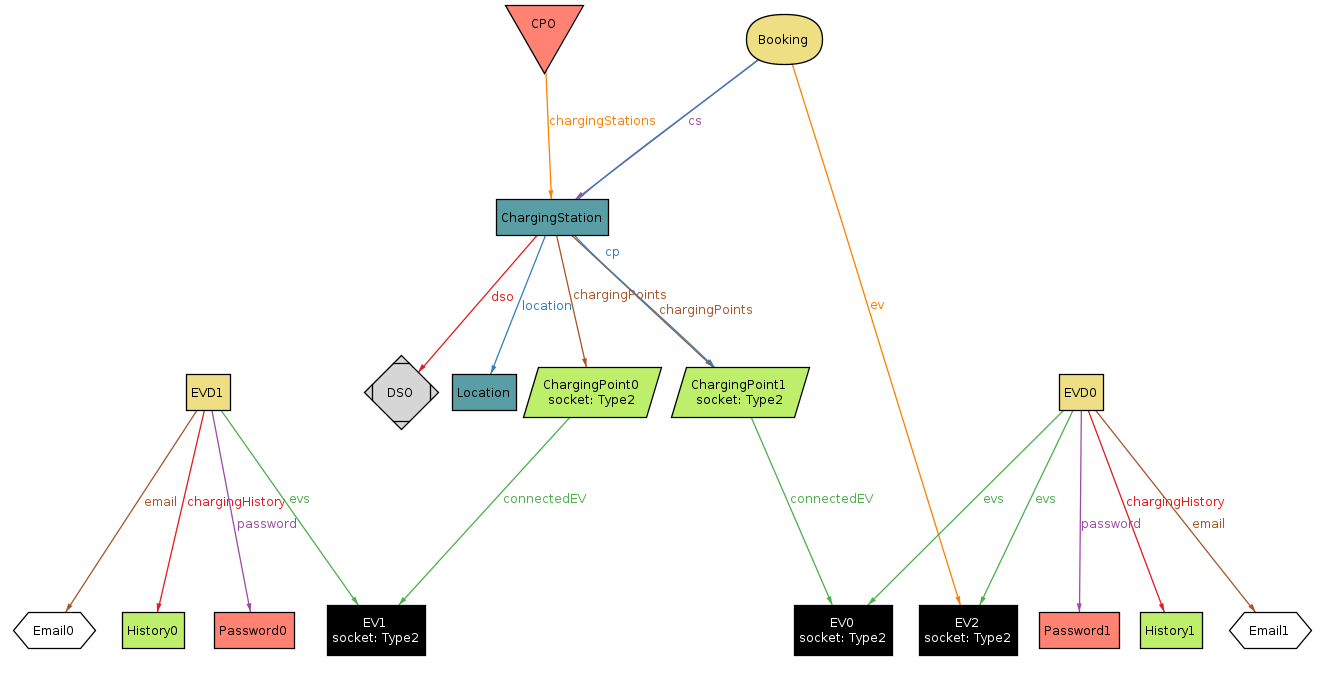
\includegraphics[width=1\textwidth]{Images/cp4/EVDWorldWithBookingAndChargeNow.png}
    \caption{A second representation of the world from the EVD point of view}
\end{figure}

Finally, we chose to show a dynamic model regarding the world that involves mainly the CPO. Running the predicate showAddCPToCS, explained in the Alloy code, we can see that a charging point is correctly added to the charging station related to the CPO that manages it.
\begin{figure}[H]
    \centering
    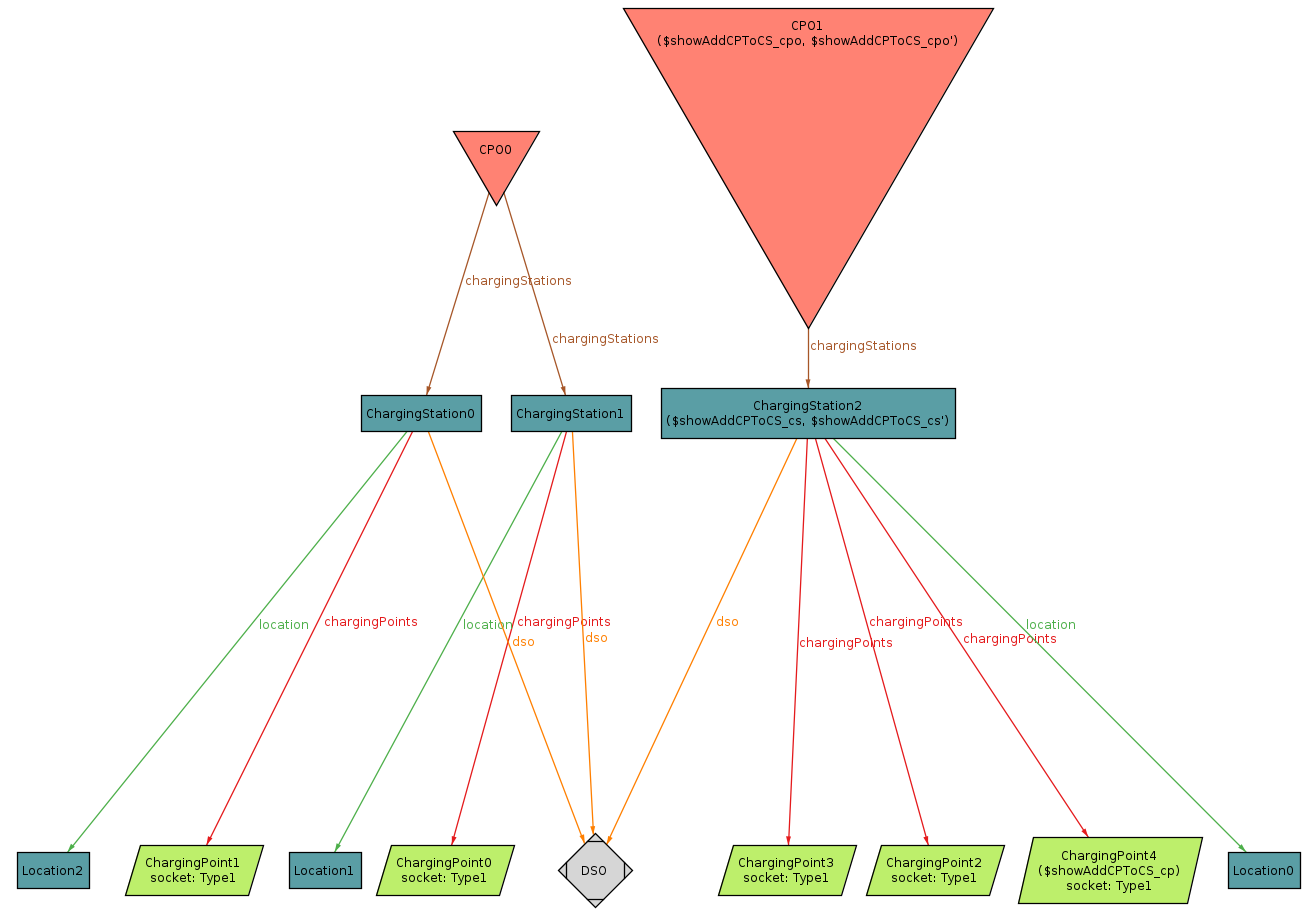
\includegraphics[width=1\textwidth]{Images/cp4/DynamicWorldAddCPToCS.png}
    \caption{A dynamic representation, considering the task of the CPO that ads a new charging point to a charging station}
\end{figure}

\chapter{Effort spent}
\label{ch:chapter_five}%
\label{sec:Effort spent}%
\begin{table}[h!]
    \centering
    \begin{tabular}{|l|c|}
     \hline
     \textbf{Activity} & \textbf{Time spent} \\
    \hline
    Organization & 5h \\
    \hline
    Understanding the problem & 10h \\
    \hline
    Introduction to the problem & 10h \\
    \hline
    Scenarios and overall description & 10h \\
    \hline
    Functional and non-functional requirements & 22h \\
    \hline
    Formal analysis using Alloy & h \\
    \hline
    Total time spent & h \\
    \hline
\end{tabular}
    \caption{The time Bianca Savoiu has spent working on this project}
    \label{tab:Assumptions}
\end{table}


\begin{table}[h!]
    \centering
    \begin{tabular}{|l|c|}
    \hline
     \textbf{Activity} & \textbf{Time spent} \\
    \hline
    Organization & 5h \\
    \hline
    Understanding the problem & 10h \\
    \hline
    Introduction to the problem & 10h \\
    \hline
    Scenarios and overall description & 8h \\
    \hline
    Functional and non-functional requirements & 12h \\
    \hline
    Formal analysis using Alloy & h \\
    \hline
    Total time spent & h \\
    \hline
\end{tabular}
    \caption{The time Fabio Lusha has spent working on this project}
    \label{tab:Assumptions}
\end{table}

\chapter{References}

\nocite{*}
%\bibliographystyle{plain}
\bibliography{bibliography}
\label{ch:chapter_six}%

% LIST OF FIGURES
\listoffigures
 
% LIST OF TABLES
\listoftables
\cleardoublepage
\end{document}
